\chapter{Understanding Personal Clouds}

Personal Clouds are complex infrastructures involving a variety of distributed components. 
Even for setting up and running a basic service, engineers in charge of building it need 
to implement many processes. The lack of a reference open source implementation complicates
even more the design of these systems. 

To put in perspective, we describe next the typical interactions among the
different blocks of a Personal Cloud architecture. Among the three key services, here we will
focus only on the synchronization service. The sharing service can be considered as a
particular case of file synchronization where users set sharing controls at the account
level to grant access of shared folders and links to other users. On the other hand, the
storage service must offer a clean and simple file-system interface for archiving, backup,
and even primary storage of files, abstracting away the complexities of direct hardware
management. At the same time, the storage service must guarantee the availability of data
files stored by users, which is achieved by adding redundancy to multiple servers. As the
implementation of the storage service is more related to hardware issues like redundancy
management, and it is in general not architecturally relevant, discussion on the storage
service has been skipped due to space constraints.


It must be noted that Personal Clouds usually treat differently desktop clients in PCs and
laptops from mobile and Web clients. Whereas the former maintain a copy of the information
and check for changes, mobile clients use to retrieve the information on demand. We will focus
only on the desktop scenario.

\subsection{Basic Blocks and Interactions}

Personal Clouds usually provide desktop clients that integrate with the OS file explorer capabilities. 
These clients include a \texttt{Watcher} component that monitors file changes in a specified 
synced folder. We will call this working folder the \textit{Workspace}.

~When the \texttt{Watcher} is notified of any change in the Workspace by the OS, it then informs 
the \texttt{Indexer} component on the new changes.  The \texttt{Indexer} maintains a local database 
with information about the contents of the Workspace including files, folders, hashes, and even versions. 
Internally, Personal Clouds typically do not use the concept of file, but rather operate on a lower level by splitting
files into chunks, each treated as independent object and identified by a fingerprint (like SHA-256 hash~\cite{drago2012inside}). 
In that case, the local database maps the fingerprints to the corresponding files. The reason to work
at the sub-file level is to transfer to the \texttt{Storage back-end}~(Dropbox uses Amazon S3 as storage back-end) only 
those parts of files that have been modified since the last synchronization, saving traffic and storage costs.

The component responsible for partitioning files and calculating the hash values is the \texttt{Chunker}.
The system could either use fixed-sized chunks or variable-sized chunks \cite{Muthitacharoen01}. Either way,
when a new file is added into the Workspace, all the new chunks will be indexed in the local database. If an existing
file is updated, only the affected chunks will be indexed. 
Once the new chunks are indexed, the \texttt{Indexer} will then apply the appropriate source-based \textit{deduplication} policy
to transfer only the unique chunks to the \texttt{Storage back-end}. If deduplication is on a per user-basis, it suffices
for the \texttt{Indexer} to compare the hashes of the new chunks with the ones in the local database. If some of the chunks already exist,
only the new ones will be uploaded to the \texttt{Storage back-end}. If deduplication is cross-user, then the \texttt{Indexer}
will have to ask first the synchronization service, \texttt{SyncService} for short, by sending to it the hash signatures of chunks.
The \texttt{SyncService} will use the hash signatures to check for the existence of chunks and then notify the \texttt{Indexer} to
upload the missing chunks to the \texttt{Storage back-end}. Here we find the first functional dependency between components, as the 
efficiency of the \texttt{Chunker} determines the amount of data to transfer to the \texttt{Storage back-end}. Ideally, only those
parts of the file that have been modified should be sent over the network, for which the choice of the chunk size is critical. 
Clearly, the best choice depends on both the number and granularity of changes. If a single character is changed in a file, 
a large-sized chunk will require transferring a lot of duplicate data, while a smaller chunk will offer a greater saving
in network bandwidth. The downside of using small chunks is that it will increase the amount of metadata to
be managed by the \texttt{SyncService}, directly impacting on the system's scalability. It is partly for this reason that an
open architecture with a modular design like StackSync can facilitate the study of these issues 
and promote further advances in the future.


\begin{figure}[t]
\centering
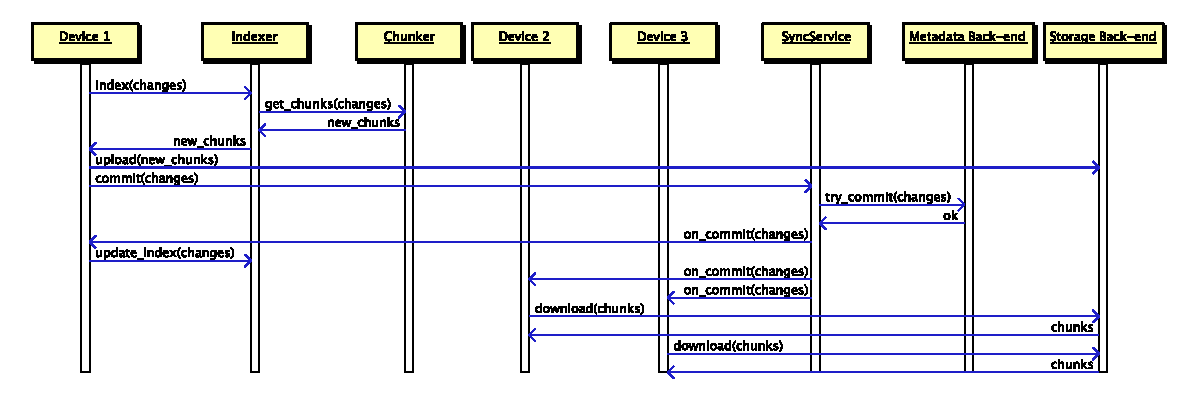
\includegraphics[width=\textwidth]{figures/stack}
\caption{Interaction between the components of sync engine for a Personal Cloud.}\label{fig:sequence}
\vspace{-10pt}
\end{figure}

Once the unique chunks are successfully submitted to the \texttt{Storage back-end}, 
the \texttt{Indexer} will communicate with the \texttt{SyncService} to commit the
changes to the \texttt{Metadata back-end}, which is the component responsible for
keeping versioning information. 
The \texttt{Metadata back-end} may be a relational
database like MySQL or a non-relational data store like Cassandra\footnote{\url{http://cassandra.apache.org/}}
or Riak\footnote{\url{http://basho.com/riak/}}, now frequently called NoSQL databases. Irrespective
of the chosen database technology, the \texttt{SyncService} needs to provide a consistent view of the synced files. 
Allowing new commit requests to see uncommitted changes may result in unwanted conflicts. As soon as more than one
user works with the same file, there is a good chance that they accidentally update their local working copies at
the same time. It is therefore critical that metadata is consistent at all times to establish not only the most
recent version of each individual file but to record its (entire) version history. Although relational databases process
data slower than NoSQL databases, NoSQL databases do not natively support ACID transactions, which could compromise
consistency, unless additional complex programming is performed. Since the nature of the \texttt{metadata back-end}
strongly determines both the scalability and complexity of the synchronization logic, an open modular architecture like StackSync
can reduce the cost of innovation, adding a great flexibility to meet changing needs.

Finally, when the \texttt{SyncService} finishes the commit operation, it will then notify of the last changes
to all out-of-sync devices. The device that originally modified the local working copy of the file will just
update the \texttt{Indexer} upon the arrival of the confirmation from the \texttt{SyncService}. 
The other devices will both update their local databases and download the new chunks from the \texttt{Storage back-end}. 
Here we are assuming that an efficient communication middleware mediates between devices and 
the \texttt{SyncService}. This middleware should support efficient marshaling and message
compression to reduce traffic overhead. Very importantly, it should support scalable change notification
to a high number of entities, using either pull or push strategies. To deduplicate files and offer continuous
reconciliation~\cite{Balasubramaniam98}, recall that the local database at the \texttt{Indexer} must
be in sync with the \texttt{Metadata back-end}, for which notification must be performed fast.

Fig.~\ref{fig:sequence} illustrates the interaction between all the components of a file sync
engine. Observe that not all the different components described in this section are present in the
architecture of a Personal Cloud. In some architectures, our overall model could be simplified and
one component could be responsible for many tasks. Some architectures can even lack some components. 
For example, ownCloud does not provide deduplication and chunking.